\documentclass[11pt, oneside, a4paper]{scrartcl}

\usepackage[english]{babel}
\usepackage[utf8x]{inputenc}

\usepackage{amssymb}
\usepackage{amsmath}
\usepackage{exscale}

\usepackage{hyperref}
\hypersetup{colorlinks=true, linkcolor=black, filecolor=black, citecolor=black, urlcolor=blue, pdfauthor = Evgeny Yulyugin, pdftitle=mipt-smb-search guide}

\usepackage{url}

\usepackage{listings}
\lstset{basicstyle=\footnotesize\ttfamily, breaklines=true, keepspaces=true }

\usepackage{subfigure}
\usepackage{graphicx}
\graphicspath{{./images/}}

\begin{document}

\title{mipt-smb-search}

\author{Yulyugin Evgeny (yulyugin@gmail.com) \\
Morgen Matvey (melges.morgen@gmail.com) \\
and others.}

\maketitle

\section{Description}

Project to write search engine for mipt campus network with video preview. Our web-cite \url{http://code.google.com/p/mipt-smb-search/}.

SVN: \url{https://mipt-smb-search.googlecode.com/svn/trunk}

\section{Dependencies}

\begin{itemize}
  \item g++-4.7
  \item libmysql++
  \item libsmbclient
  \item libprocps
  \item libcppunit
  \item libmagic
\end{itemize}

\section{How to build}\label{sec:build}

\subsection{Build with Qt-Creator}

When you open Qt-Creaotr at first you can see window like fig.~\ref{fig:qt-creator-config-main}. Clear "Shadow build".

\begin{figure}[ht]
  \centering
  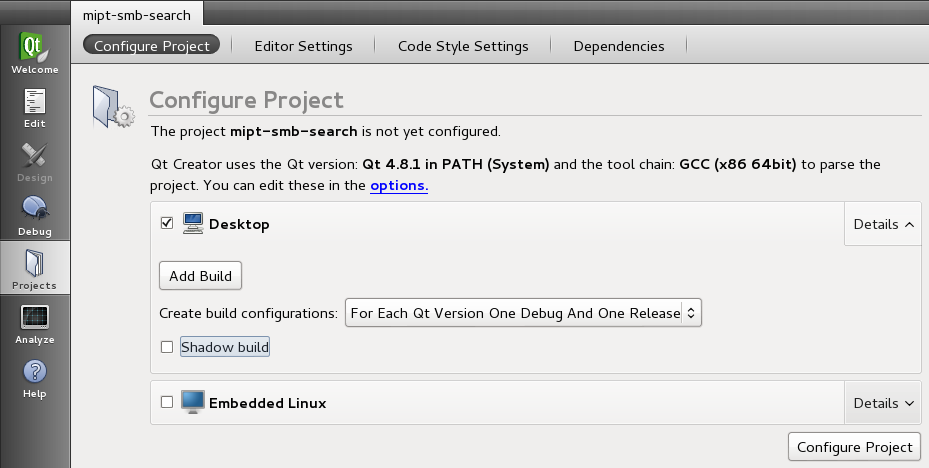
\includegraphics[width=0.8\textwidth]{./qt-creator-config-main.png}
  \caption{Qt-Creator settings main.}
  \label{fig:qt-creator-config-main}
\end{figure}

Release setting should look like fig~\ref{fig:qt-creator-config-release}. Debug setting should look like fig~\ref{fig:qt-creator-config-debug}.

\begin{figure}[ht]
  \centering
  \subfigure[]{
    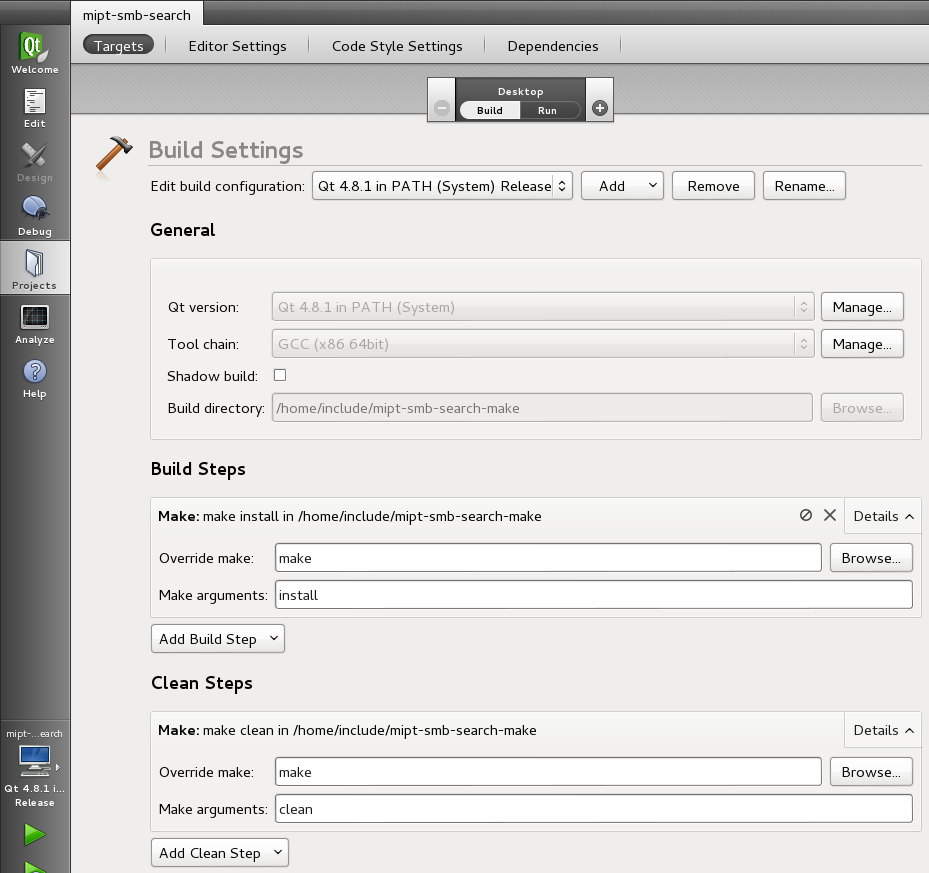
\includegraphics[width=0.8\textwidth]{./qt-creator-config-build-release.png}
    \label{fig:qt-creator-config-release}
  }
  \subfigure[]{
    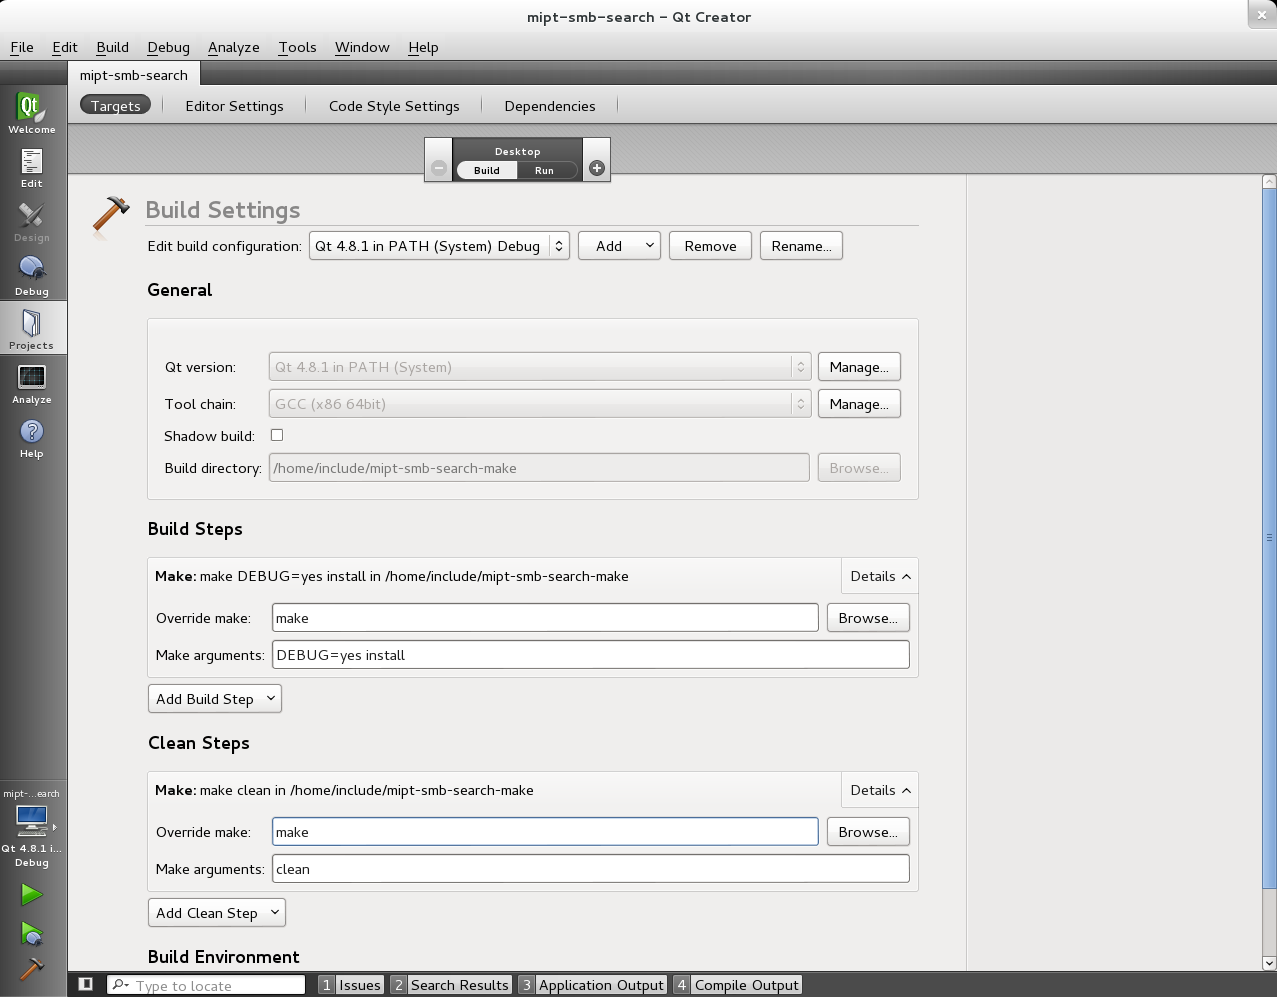
\includegraphics[width=0.8\textwidth]{./qt-creator-config-build-debug.png}
    \label{fig:qt-creator-config-debug}
  }
  \caption{Build settings for Qt-Creator: \subref{fig:qt-creator-config-release} for release build, \subref{fig:qt-creator-config-debug} for debug build.}
\end{figure}

\subsection{Build without Qt-Creator}

By default project will build in svn\_dir/build/release in release mode and svn\_dir/build/debug in debug mode.

\begin{lstlisting}
$ make install
\end{lstlisting}

To build in debug mode you should use next command:

\begin{lstlisting}
$ make DEBUG=yes install
\end{lstlisting}

\section{How to run tests}\label{sec:tests}

\subsection{Without Qt-Creator}

\begin{lstlisting}
$ ./mipt-smb-search/tests/testing.sh <path_to_build_directory>
\end{lstlisting}

\subsection{With Qt-Creator}

This is an example of Qt-Creator settings to run fulltest. This settings should be done after build settings (look at section~\ref{sec:build} for more details).

\begin{enumerate}
  \item First of all you should choose pass to executable file. In our example it's situated in \%{buildDir}/build/debug/tests/bin/fulltest
  \item Than add path to working directory. Full test should executes from directory when it situates. In our example it's situated in \%{buildDir}/build/debug/tests/bin
  \item You should set LD\_LIBRARY\_PATH variable to detect new shared libraries which created in our project. You should add path to lib and tests/lib folder. LD\_LIBRARY\_PATH should contain full path to this folder.
\end{enumerate}

The result of this settings could be shown in fig.~\ref{fig:qt-creator-config-run}

\begin{figure}[ht]
  \centering
  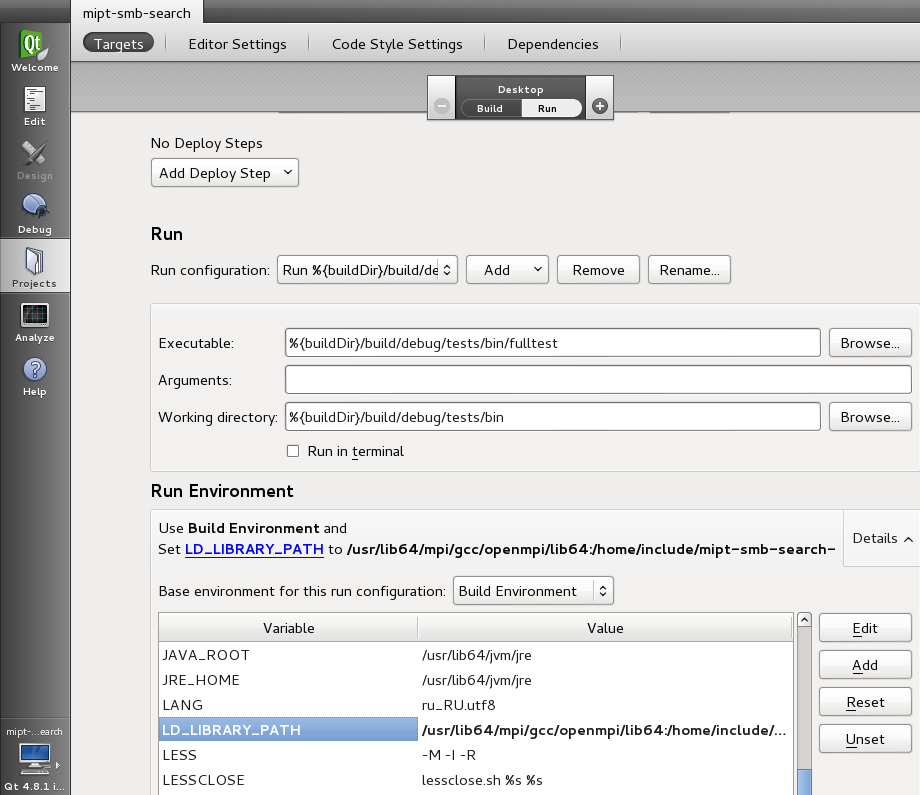
\includegraphics[width=0.8\textwidth]{./qt-creator-config-run.png}
  \caption{Qt-Creator settings to run.}
  \label{fig:qt-creator-config-run}
\end{figure}

You can configure run settings for each executable file based on this algorithm.

\section{Coading style}

We use google coading style for more details see "Google C++ Style Guide" (\url{http://google-styleguide.googlecode.com/svn/trunk/cppguide.xml}) for C++ codes.

\section{How to commit changes}

Before commit your changes you should pass code review.

To send your patch on code review you should use upload.py script (\url{https://codereview.appspot.com/static/upload.py}).

\begin{lstlisting}
$ python2.7 upload.py -m "My important change description."
\end{lstlisting}

For more imformation about usage and option of upload.py see \url{http://code.google.com/p/rietveld/wiki/UploadPyUsage}.

Then go to \url{https://codereview.appspot.com/}, choose your subject.

Reviewers: yulyugin@gmail.com, melges.morgen@gmail.com

CC: mipt-smb-search-review@googlegroups.com

Description: Description of your changes and testlog.

Than start codereview review.

After "LGTM" you can commit your changes.

\begin{lstlisting}
svn commit -m "My importand change description."
\end{lstlisting}

\section{How to write tests}

\section{How to test coverage}

\begin{enumerate}
  \item Build with TEST\_COVERAGE flag:
\begin{lstlisting}
$ make TEST_COVERAGE=yes
\end{lstlisting}
  \item Run tests. For more information see section~\ref{sec:tests}
  \item Go to the directory with tested file.
\begin{lstlisting}
$ cd mipt-smb-serach/spider
\end{lstlisting}
  \item Test coverage with gcov programm
\begin{lstlisting}
$ gcov spider.gcda
File 'mipt-smb-search/spider/spider.cpp'
Lines executed:55.23% of 239
Creating 'spider.cpp.gcov'
\end{lstlisting}
  \item You can see information about what lines and how often been executed.
\begin{lstlisting}
$ nano spider.cpp.gcov
\end{lstlisting}
\end{enumerate}

\end{document}

